\documentclass[12pt,a4paper]{article}
\usepackage[T1]{fontenc}
\usepackage[utf8]{inputenc}
\usepackage[french]{babel}
\usepackage{lmodern}
\usepackage[a4paper,margin=1.7cm,top=1.4cm,bottom=1.5cm]{geometry}
\usepackage{amsmath}
\usepackage{booktabs}
\usepackage{graphicx}
\usepackage{xcolor}
\usepackage[font=small,labelfont=bf,skip=3pt]{caption}
\usepackage{microtype}
\usepackage[hidelinks]{hyperref}
\usepackage{enumitem}

% ---- Lien vers le code source (à remplacer par le lien GitHub ou Colab partagé) ----
\newcommand{\lienCode}{\url{https://github.com/Harena21/tp-clip}}

\setlength{\parskip}{2pt}
\setlength{\parindent}{0pt}
\setlength{\abovedisplayskip}{3pt}
\setlength{\belowdisplayskip}{3pt}
\renewcommand{\arraystretch}{1.05}
\setlength{\tabcolsep}{4pt}
\pagestyle{plain}

\newcommand{\sect}[1]{\vspace{4pt}{\large\bfseries #1}\par\vspace{1pt}}

\begin{document}

\begin{center}
{\Large\bfseries Représentations multimodales texte/image avec CLIP}\\[2pt]
TP de Multi-modalité et IA générative (IFLCE055), M2 VMI, Université Paris Cité\\[1pt]
Lucka Harena \quad--\quad 21 novembre 2026\\[1pt]
Code source (notebook Colab commenté) : \lienCode
\end{center}

\sect{1. Méthode et état d'avancement}
CLIP~\cite{radford} apprend un encodeur d'image et un encodeur de texte qui projettent leurs entrées dans un même espace. L'entraînement porte sur 400~M de paires image/texte du web avec une loss contrastive symétrique~\cite{cours} : dans un batch de $N$ paires d'embeddings normalisés $(v_i,u_i)$, chaque image doit être plus proche de sa légende que des $N-1$ autres,
\begin{equation*}
\mathcal{L}=\tfrac{1}{2N}\textstyle\sum_{i}\Big[-\log\frac{e^{\langle v_i,u_i\rangle/\tau}}{\sum_j e^{\langle v_i,u_j\rangle/\tau}}-\log\frac{e^{\langle u_i,v_i\rangle/\tau}}{\sum_j e^{\langle u_i,v_j\rangle/\tau}}\Big].
\end{equation*}
En zero-shot, une image est classée en la comparant aux embeddings de phrases du type \og a photo of a \{classe\}\fg.
Les quatre consignes sont traitées. Le tutoriel~\cite{tuto} a été exécuté en entier sur Colab (GPU T4), fine-tuning compris, puis j'ai ajouté une partie évaluation à la fin du notebook. Toutes les métriques sont sauvegardées dans un fichier JSON. J'évalue la recherche image$\leftrightarrow$texte par le Recall@K, noté R@K, comme pour COCO dans le cours~\cite{cours} : c'est la part des requêtes dont la bonne réponse se trouve parmi les K premiers résultats. La classification est évaluée par la précision top-1 et top-5.

\sect{2. Prise en main du tutoriel (consigne 1)}
Sur les 8 images naturelles, ViT-B/16 retrouve les 8 bonnes descriptions dans les deux sens. La similarité moyenne vaut 0,31 pour les bonnes paires et 0,16 pour les mauvaises, soit un écart de 0,151. Sur les 8 images ROCO, il n'en retrouve que 5/8 (image$\to$texte) et 7/8 (texte$\to$image), avec un écart de 0,056. Les bonnes paires médicales ne sont pas moins similaires (0,32) : ce sont les mauvaises paires qui le sont beaucoup plus (0,26). Les légendes contenant \og CT\fg{} sont proches de toutes les coupes, scanners comme IRM, ce qui suggère que CLIP repère le type d'examen plus que la lésion.
En lisant le code, j'ai relevé deux points. La démo zero-shot CIFAR-100 réutilise les embeddings des images médicales : CLIP doit alors choisir entre \og turtle\fg, \og plate\fg{} ou \og baby\fg{} pour un scanner, avec des probabilités sous 0,35, ce qui illustre que le softmax force un choix même sans classe pertinente. La boucle de fine-tuning contient un \texttt{return} avant la validation. Elle s'arrête donc après une époque (loss contrastive de 1,60 à 0,33, pour $\ln 16\approx2{,}77$ au hasard) sans écrire de checkpoint, et la suite utilise le checkpoint fourni.

\sect{3. Comparaison des 9 modèles CLIP (consigne 2)}
\texttt{clip.available\_models()} propose 5 ResNet modifiés (RN50, RN101 et RN50x4/x16/x64, agrandis en largeur, profondeur et résolution) et 4 ViT~\cite{vit} (B/32, B/16, L/14, et L/14@336px qui est le même L/14 avec des images de 336 pixels ; le nombre après la barre est la taille des patchs). J'ai évalué chacun avec le même protocole : classification zero-shot sur CIFAR-100~\cite{cifar} avec le prompt \og a photo of a \{classe\}.\fg{} et recherche image$\leftrightarrow$texte sur 1\,000 paires de validation de ROCO~\cite{roco} tirées avec une graine fixe (hasard : R@1 = 0,1\,\%).

\begin{table}[h]
\centering\footnotesize
\caption{Les 9 modèles CLIP. C100 : CIFAR-100 zero-shot (top-1/top-5, \%), « Art. » : top-1 publié~\cite{radford} (tab.~11). ROCO : Recall@K (\%) sur 1\,000 paires. Temps : ms/image sur T4.}
\label{tab:modeles}
\begin{tabular}{lrrrrrrrrr}
\toprule
Modèle & Param. (M) & Rés. & ms/img & C100 top-1 & top-5 & Art. & i$\to$t R@1 & i$\to$t R@10 & t$\to$i R@10\\
\midrule
RN50 & 102 & 224 & 2,2 & 40,5 & 72,7 & 41,6 & 4,5 & 20,8 & 19,1\\
RN101 & 120 & 224 & 2,5 & 46,9 & 76,4 & 49,0 & 4,4 & 20,7 & 21,1\\
RN50x4 & 178 & 288 & 5,1 & 42,5 & 71,7 & 48,9 & 5,3 & 25,4 & 26,1\\
RN50x16 & 291 & 384 & 13,4 & 48,8 & 75,8 & 54,2 & 7,4 & 28,2 & 28,4\\
RN50x64 & 623 & 448 & 38,5 & 55,7 & 81,1 & 61,3 & 8,9 & 33,6 & 31,6\\
ViT-B/32 & 151 & 224 & 2,0 & 62,3 & 86,9 & 65,1 & 4,7 & 21,8 & 19,0\\
ViT-B/16 & 150 & 224 & 3,1 & 67,2 & 89,1 & 68,7 & 7,1 & 26,9 & 25,1\\
ViT-L/14 & 428 & 224 & 12,0 & \textbf{76,0} & \textbf{93,4} & 77,9 & 9,4 & 34,8 & 31,4\\
ViT-L/14 (336 px) & 428 & 336 & 29,0 & 75,7 & 93,3 & 77,5 & \textbf{10,1} & \textbf{35,4} & \textbf{33,7}\\
\bottomrule
\end{tabular}
\end{table}

Sur CIFAR-100, les ViT sont nettement meilleurs à coût égal : ViT-B/32 dépasse RN50 de 22 points pour un temps d'encodage identique (figure~\ref{fig:modeles}). Passer L/14 en 336 pixels ne gagne rien et coûte 2,4 fois plus de temps, ce qui est logique pour des images de 32$\times$32 pixels agrandies. Nos scores sont 1 à 6,5 points sous ceux de l'article. L'article combine plusieurs prompts~\cite{radford} alors que j'en utilise un seul, et par oubli de \texttt{train=False} l'évaluation a porté sur les 50\,000 images d'entraînement de CIFAR-100 au lieu du test (sans incidence sur le caractère zero-shot, mais les chiffres ne sont pas strictement comparables). Sur ROCO, tous les modèles restent faibles (R@1 $\le$ 10\,\%) et le classement change : RN50x16 et RN50x64 dépassent ViT-B/16 en R@10 malgré 18 et 11 points de moins sur CIFAR. Comme ils travaillent en 384 et 448 pixels, je suppose que la résolution aide pour les détails fins des radiographies. ViT-L/14 offre le meilleur compromis global, ViT-B/16 le meilleur pour un budget de calcul serré.

\begin{figure}[h]
\centering
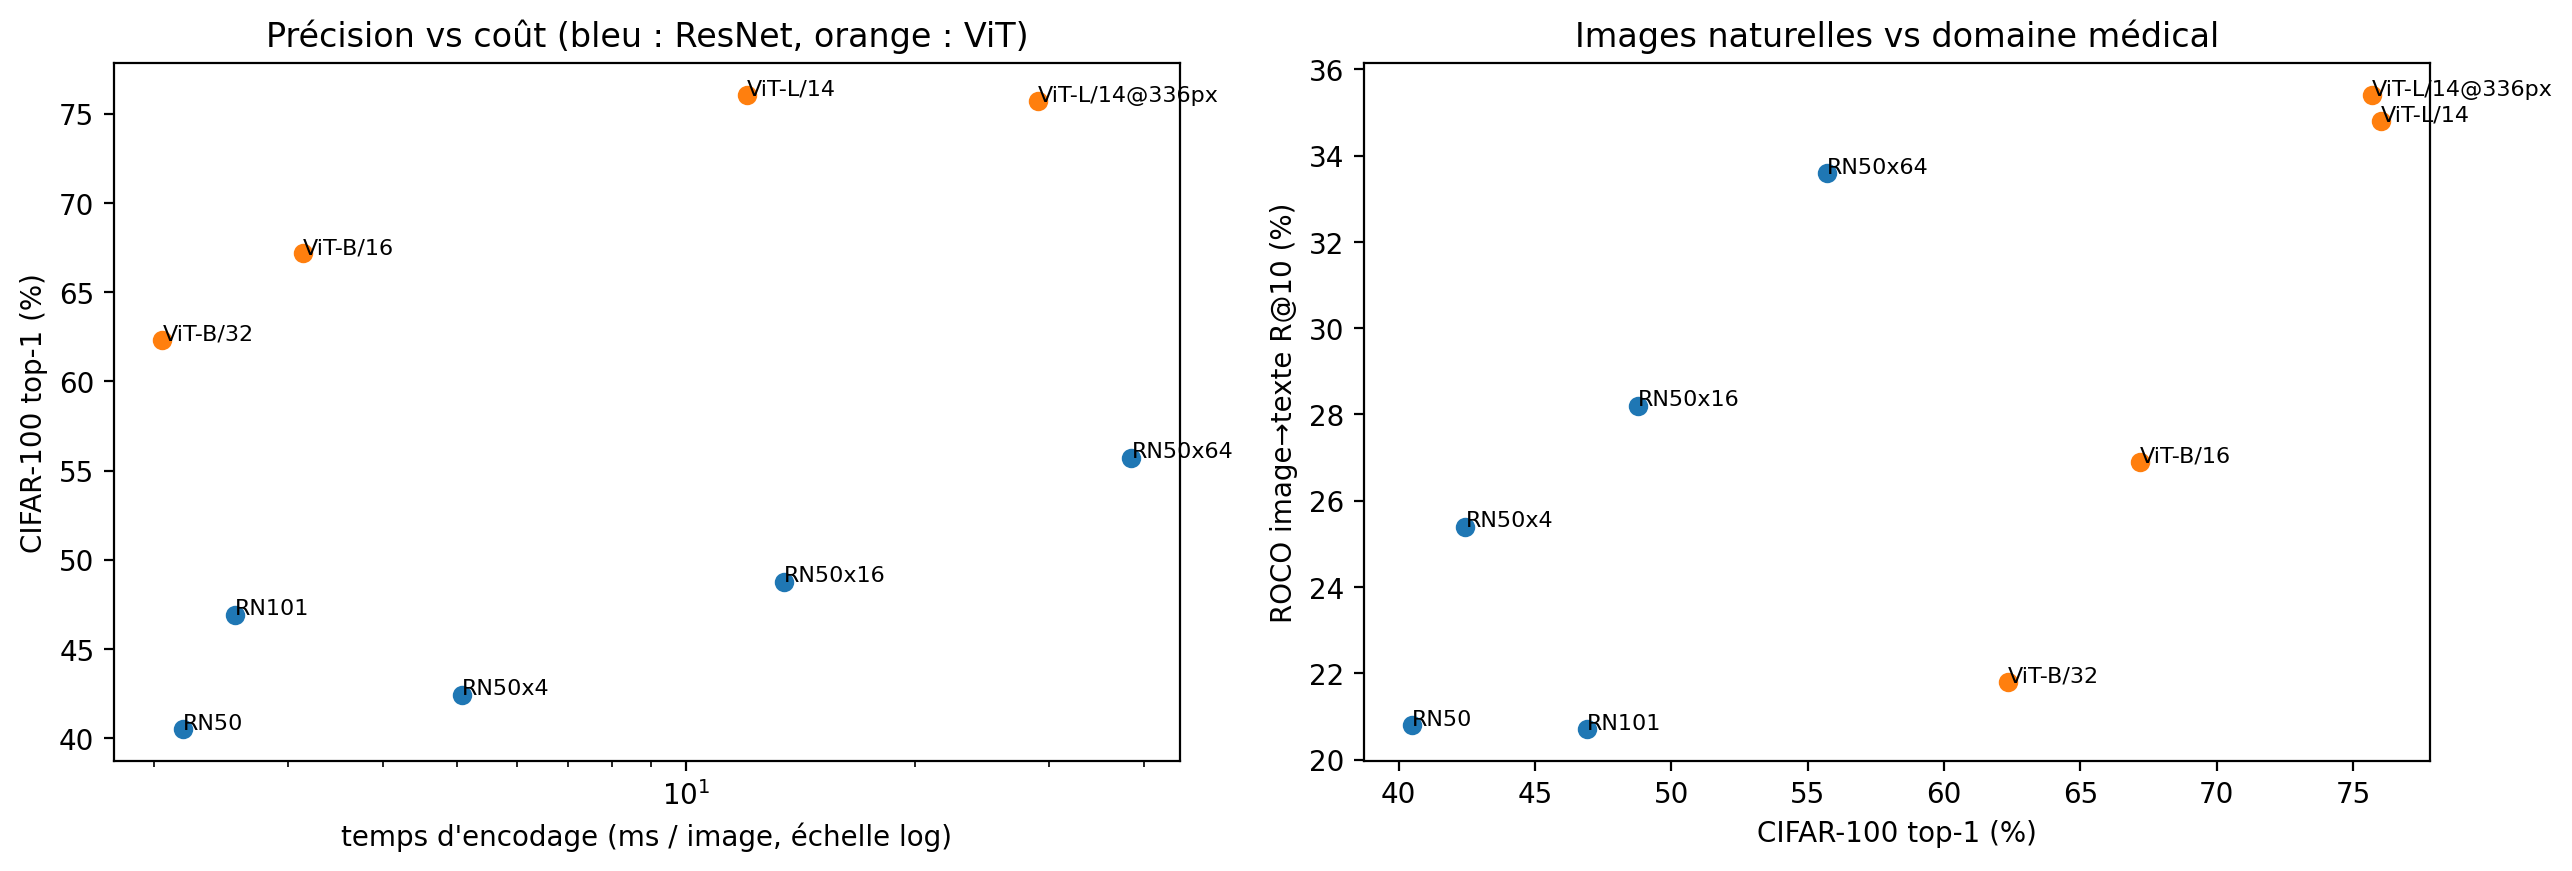
\includegraphics[width=0.8\linewidth]{fig_modeles.png}
\caption{À gauche : précision CIFAR-100 en fonction du temps d'encodage (bleu : ResNet, orange : ViT). À droite : CIFAR-100 contre ROCO R@10, les deux classements ne coïncident pas.}
\label{fig:modeles}
\end{figure}

\sect{4. CLIP dans le domaine médical (consigne 3)}
J'ai comparé ViT-B/16 zero-shot et ViT-B/16 fine-tuné sur ROCO (checkpoint fourni) sur trois tâches, toujours avec des images de validation : 8 nouveaux exemples tirés au hasard, la recherche sur les 1\,000 paires, et la classification zero-shot de la modalité d'imagerie. Pour cette dernière, l'étiquette est extraite de la légende par expressions régulières, en ne gardant que les légendes citant une seule modalité (626 images : 231 CT, 118 IRM, 164 radiographies, 74 échographies, 39 angiographies ; prédire toujours \og CT\fg{} donne 36,9\,\%).

\begin{table}[h]
\centering\footnotesize
\caption{ViT-B/16 avant et après fine-tuning sur ROCO (images de validation). Modalité : top-1 et précision moyenne par classe (\%).}
\label{tab:medical}
\begin{tabular}{lcccccc}
\toprule
& 8 ex. (i$\to$t, t$\to$i) & i$\to$t R@1 & i$\to$t R@10 & t$\to$i R@1 & t$\to$i R@10 & Modalité (top-1 / moy.)\\
\midrule
Zero-shot & 6/8 \; 7/8 & 7,1 & 26,9 & 5,8 & 25,1 & 73,2 / 75,1\\
Fine-tuné ROCO & 8/8 \; 8/8 & \textbf{27,6} & \textbf{69,4} & \textbf{26,4} & \textbf{69,8} & \textbf{96,2} / \textbf{97,4}\\
\bottomrule
\end{tabular}
\end{table}

Le fine-tuning multiplie le R@1 par quatre. En zero-shot, les erreurs sur les 8 exemples portent sur deux images dentaires confondues entre elles et sur la légende \og Preoperative OPG\fg, dont toutes les similarités restent entre 0,22 et 0,28 : CLIP ne connaît visiblement pas cette abréviation. La modalité est déjà reconnue dans 73\,\% des cas sans aucun apprentissage. Les radiographies sont presque parfaites (162/164), mais \og angiography\fg{} attire 61 scanners et 30 échographies, et 30 IRM sont prises pour des scanners (figure~\ref{fig:modalite}). Après fine-tuning, il reste surtout 13 scanners classés IRM. CLIP généraliste identifie donc le type d'examen mais pas le contenu clinique de la légende. Une partie des échecs en recherche vient aussi des faux négatifs évoqués en cours~\cite{cours} : beaucoup de légendes ROCO sont presque interchangeables (\og CT scan of the chest\dots\fg).

\begin{figure}[h]
\centering
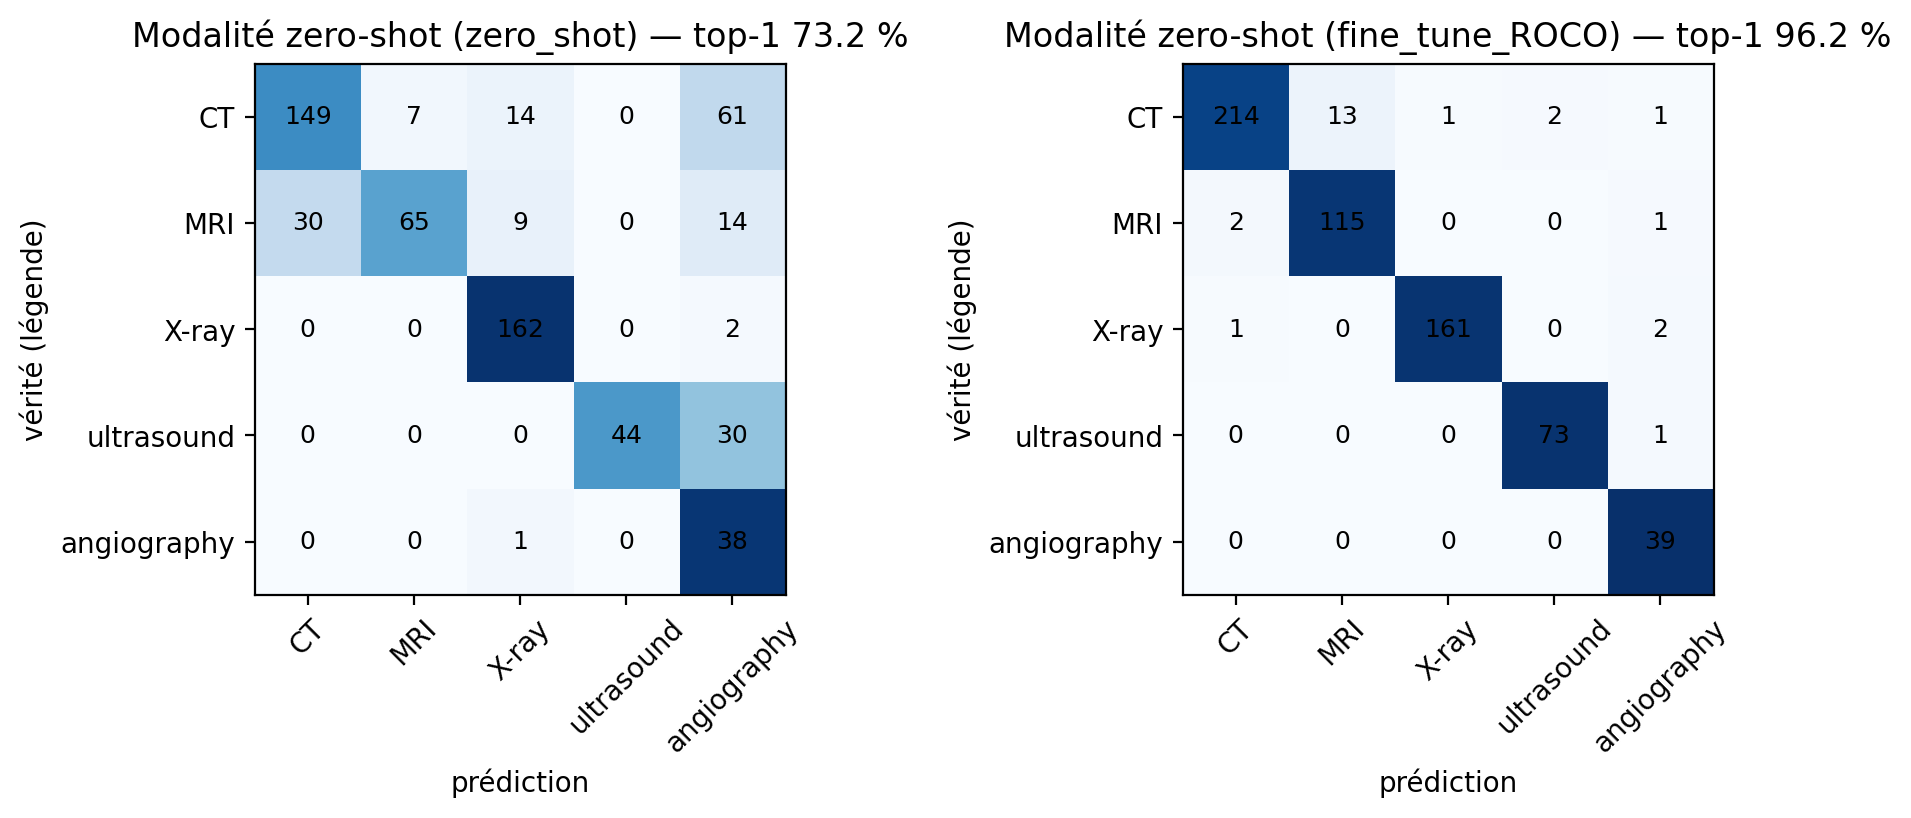
\includegraphics[width=0.6\linewidth]{fig_modalite.png}
\caption{Matrices de confusion de la modalité (lignes : vérité issue de la légende), zero-shot à gauche et fine-tuné à droite.}
\label{fig:modalite}
\end{figure}

\sect{5. Classification d'images naturelles : Oxford-IIIT Pet (consigne 4)}
J'ai choisi Oxford-IIIT Pet~\cite{pets} (37 races de chats et de chiens, 3\,669 images de test) parce que c'est une classification fine, très différente de CIFAR-100, et que l'article CLIP donne des chiffres de référence pour ce jeu. Deux prompts sont comparés : (A) \og a photo of a \{race\}.\fg{} et (B) \og a photo of a \{race\}, a type of pet.\fg, proposé par Radford et al.~\cite{radford} pour lever l'ambiguïté de noms comme \og Boxer\fg.

\begin{table}[h]
\centering\small
\caption{Oxford-IIIT Pet zero-shot (\%, split de test). Moy./classe : métrique officielle du jeu ; Art. : valeur publiée~\cite{radford}.}
\label{tab:pets}
\begin{tabular}{lcccccc}
\toprule
Modèle & Top-1 (A) & Top-1 (B) & Top-5 (B) & Moy./classe (B) & Art. & Gain B$-$A\\
\midrule
RN50 & 83,7 & 85,7 & 99,2 & 85,5 & 85,4 & +2,1\\
RN101 & 84,9 & 86,9 & 99,0 & 86,6 & 86,2 & +2,0\\
ViT-B/32 & 85,0 & 87,4 & 99,3 & 87,1 & 87,0 & +2,4\\
ViT-B/16 & \textbf{88,3} & \textbf{89,1} & \textbf{99,5} & \textbf{88,9} & 88,9 & +0,8\\
\bottomrule
\end{tabular}
\end{table}

CLIP atteint 89,1\,\% de top-1 sans voir une seule image d'entraînement, et nos précisions moyennes par classe sont à moins de 0,5 point de l'article, ce qui valide le protocole. Le prompt avec contexte apporte 0,8 à 2,4 points. Les erreurs de ViT-B/16 portent sur des races presque identiques : 45 Sacrés de Birmanie classés Ragdoll (et 20 dans l'autre sens), 22 American Pit Bull Terriers classés Staffordshire. La pire classe est Bombay (27\,\%), un chat noir ; le nom désigne aussi une ville, ce qui pourrait gêner l'encodeur de texte, mais je ne l'ai pas vérifié.

\sect{6. Limites}
Chaque mesure repose sur une seule exécution et un seul échantillon de 1\,000 paires ROCO. Les étiquettes de modalité sont bruitées. Le checkpoint fine-tuné, nommé \og best\fg, a sans doute été choisi sur ce même fichier de validation, ce qui peut rendre le gain un peu optimiste. Enfin, CIFAR-100 devrait être réévalué sur son split de test avec \texttt{train=False}.

\vspace{3pt}
\renewcommand{\refname}{\normalsize Références}
\begin{thebibliography}{9}\footnotesize\setlength{\itemsep}{0pt}
\bibitem{radford} A. Radford \textit{et al.}, \textit{Learning Transferable Visual Models From Natural Language Supervision}, ICML 2021, arXiv:2103.00020.
\bibitem{cours} Cours 1, \textit{Multimodal Deep Learning}, UE Multi-modalité et IA générative, M2 VMI, Université Paris Cité, 2026 (diapositives 34--35 : loss contrastive et CLIP ; 43 : faux négatifs ; 74 : COCO et image-caption retrieval).
\bibitem{tuto} C. Kurtz, X. Wei, \textit{CLIP tutorial (with medical images ROCO)}, \url{https://github.com/ckurtz/teaching_UPC_UFRMI}.
\bibitem{roco} O. Pelka \textit{et al.}, \textit{Radiology Objects in COntext (ROCO): A Multimodal Image Dataset}, workshops MICCAI (LABELS), LNCS 11043, 2018.
\bibitem{vit} A. Dosovitskiy \textit{et al.}, \textit{An Image is Worth 16x16 Words: Transformers for Image Recognition at Scale}, ICLR 2021.
\bibitem{cifar} A. Krizhevsky, \textit{Learning Multiple Layers of Features from Tiny Images}, rapport technique, Université de Toronto, 2009.
\bibitem{pets} O. M. Parkhi, A. Vedaldi, A. Zisserman, C. V. Jawahar, \textit{Cats and Dogs}, CVPR 2012.
\end{thebibliography}

\end{document}
